\documentclass[10pt,a4paper]{article}
\usepackage[margin=10mm,top=8mm,bottom=9mm]{geometry}
\usepackage{amsmath,amssymb}
\usepackage{booktabs}
\usepackage{tabularx}
\usepackage{graphicx}
\usepackage{enumitem}
\usepackage{microtype}
\usepackage[T1]{fontenc}
\usepackage[utf8]{inputenc}
\usepackage{lmodern}
\usepackage{xcolor}
\usepackage{tcolorbox}
\usepackage{url}

\pagestyle{empty}
\setlength{\parindent}{0pt}
\setlength{\parskip}{0.10em}

\newcolumntype{L}[1]{>{\raggedright\arraybackslash}p{#1}}
\newcolumntype{C}[1]{>{\centering\arraybackslash}p{#1}}
\newcolumntype{R}[1]{>{\raggedleft\arraybackslash}p{#1}}

\begin{document}

% ==================== PAGE 1 ====================
\begin{center}
  {\Large\textbf{Master Thesis Supervisor Executive Decision Sheet}}\\[0.18em]
  {\large\textbf{Mode-I Adaptive Remeshing Spatial Localization: Diagnosis \& Baseline Selection}}\\[0.12em]
  {\normalsize\textbf{Date:} Thursday, 08 October 2026, 10:00 \quad $\cdot$ \quad \textbf{Meeting Duration:} 45 Minutes}\\[0.08em]
  {\footnotesize\textbf{Candidate:} Pruthviraja Reddy Vandavagali (Matr. Nr. 68865) \quad $\cdot$ \quad \textbf{Supervisors:} Prof. B.~Kiefer, Dr.~S.~Roth (IMFD)}
\end{center}
\vspace{-0.45em}
\hrule height 0.7pt
\vspace{0.2em}

\begin{tcolorbox}[colback=blue!5!white,colframe=blue!60!black,title=\textbf{Governing Directive \& Active Phase},top=2pt,bottom=2pt,left=4pt,right=4pt]
\centering
\small\emph{``We need to have understood everything related to the first model before we increase complexity.''} \quad $\cdot$ \quad \textbf{Active Phase:} \texttt{MODE1\_GATE6B\_ACTIVE}
\end{tcolorbox}

\vspace{-0.25em}
\subsection*{1. Problem Observed: Downstream Coarsening in Original Adapted Mesh}
\vspace{-0.25em}
In the original Gate-5 adaptive remeshing reproduction ($48{,}329$ finite elements), the adapted mesh clustered excessively around the initial notch tip at $(x, y) = (0.50, 0.50)\,\mathrm{mm}$ and coarsened rapidly downstream along the horizontal ligament:
\begin{itemize}[itemsep=0.2pt,topsep=0.2pt,leftmargin=4mm]
  \small
  \item At initial crack tip ($x = 0.55\,\mathrm{mm}$), resolution was fine with area-equivalent size $h_A = 1.68\,\mu\mathrm{m}$.
  \item Downstream along prospective crack path: $h_A = 4.68\,\mu\mathrm{m}$ at $x = 0.65\,\mathrm{mm}$, $h_A = 5.21\,\mu\mathrm{m}$ at $x = 0.75\,\mathrm{mm}$, and $h_A = 12.58\,\mu\mathrm{m}$ at $x = 0.90\,\mathrm{mm}$ (exceeding the phase-field resolution limit $h \le l_0/2 = 3.75\,\mu\mathrm{m}$ for $l_0 = 7.5\,\mu\mathrm{m}$).
\end{itemize}

\vspace{-0.25em}
\subsection*{2. Verified Project Root Cause: Abaqus \texttt{RemeshingRule} Step Selection}
\vspace{-0.25em}
Controlled CAE diagnostics isolated the exact cause within our Python workflow:
\begin{itemize}[itemsep=0.2pt,topsep=0.2pt,leftmargin=4mm]
  \small
  \item \textbf{Step-1 Evaluation:} Evaluating \texttt{RemeshingRule} on the Step-1 linear-elastic pre-peak error field (\texttt{stepName='Step-1'}) produced stress concentration singularities exclusively at the stationary crack tip $(0.5, 0.5)\,\mathrm{mm}$. Because no crack propagated in Step 1, downstream stress gradients were smooth, causing zero refinement along the ligament.
  \item \textbf{Step-2 Evaluation:} Changing \textbf{only} the evaluated step to Step-2 crack propagation (\texttt{stepName='Step-2'}), with all sizing and indicator parameters unchanged (\texttt{MISESERI}, target $1.0\%$, $h \in [1.0, 20.0]\,\mu\mathrm{m}$, \texttt{refinementFactor=10}, whole-domain \texttt{All\_elem}), captures the propagating crack front and extends refinement along the full ligament ($62{,}057$ finite elements, $61{,}646$ nodes).
\end{itemize}

\vspace{-0.25em}
\subsection*{3. Quantitative Evidence: Step-1 vs Step-2 Candidate Comparison}
\vspace{-0.25em}
\begin{table}[h!]
  \centering
  \scriptsize
  \renewcommand{\arraystretch}{1.02}
  \begin{tabularx}{\textwidth}{L{48mm} C{22mm} C{22mm} C{18mm} X}
    \toprule
    \textbf{Geometric Metric / Location} & \textbf{Step-1 Mesh (48k)} & \textbf{Step-2 Candidate (62k)} & \textbf{Relative Change} & \textbf{Physical Impact} \\
    \midrule
    \textbf{Forward Crack Corridor} ($x \ge 0.5, |y-0.5| \le 0.05$) & $3{,}351$ elements & $\mathbf{9{,}442}$ \textbf{elements} & $\mathbf{+181.8\%}$ & $2.8\times$ element density along crack path \\
    \textbf{Crack Wake Region} ($x \le 0.5, |y-0.5| \le 0.05$) & $1{,}773$ elements & $\mathbf{428}$ \textbf{elements} & $\mathbf{-75.9\%}$ & Suppresses wasteful wake refinement \\
    \textbf{Direct Ligament Intersects} ($y \approx 0.5, x \ge 0.5$) & $150$ elements & $\mathbf{293}$ \textbf{elements} & $\mathbf{+95.3\%}$ & Double longitudinal sampling resolution \\
    \midrule
    \textbf{Median $h_A$ at Station $x = 0.55\,\mathrm{mm}$} & $1.68\,\mu\mathrm{m}$ & $\mathbf{1.89\,\mu\mathrm{m}}$ & $+12.5\%$ & Sustained within $h \le 2.0\,\mu\mathrm{m}$ ($h/l_0 \le 0.25$) \\
    \textbf{Median $h_A$ at Station $x = 0.65\,\mathrm{mm}$} & $4.68\,\mu\mathrm{m}$ & $\mathbf{1.20\,\mu\mathrm{m}}$ & $\mathbf{-74.4\%}$ & Restores fine phase-field resolution \\
    \textbf{Median $h_A$ at Station $x = 0.75\,\mathrm{mm}$} & $5.21\,\mu\mathrm{m}$ & $\mathbf{1.49\,\mu\mathrm{m}}$ & $\mathbf{-71.4\%}$ & Eliminates coarse downstream barrier \\
    \textbf{Median $h_A$ at Station $x = 0.90\,\mathrm{mm}$} & $12.58\,\mu\mathrm{m}$ & $\mathbf{3.86\,\mu\mathrm{m}}$ & $\mathbf{-69.3\%}$ & Bounded fine mesh up to boundary edge \\
    \midrule
    \textbf{Bounded Sizing Compliance} ($h \in [1, 20]\,\mu\mathrm{m}$) & $99.47\%$ & $\mathbf{99.70\%}$ & $+0.23\%$ & Strict compliance with sizing constraints \\
    \bottomrule
  \end{tabularx}
\end{table}

\vspace{-0.4em}
\begin{center}
  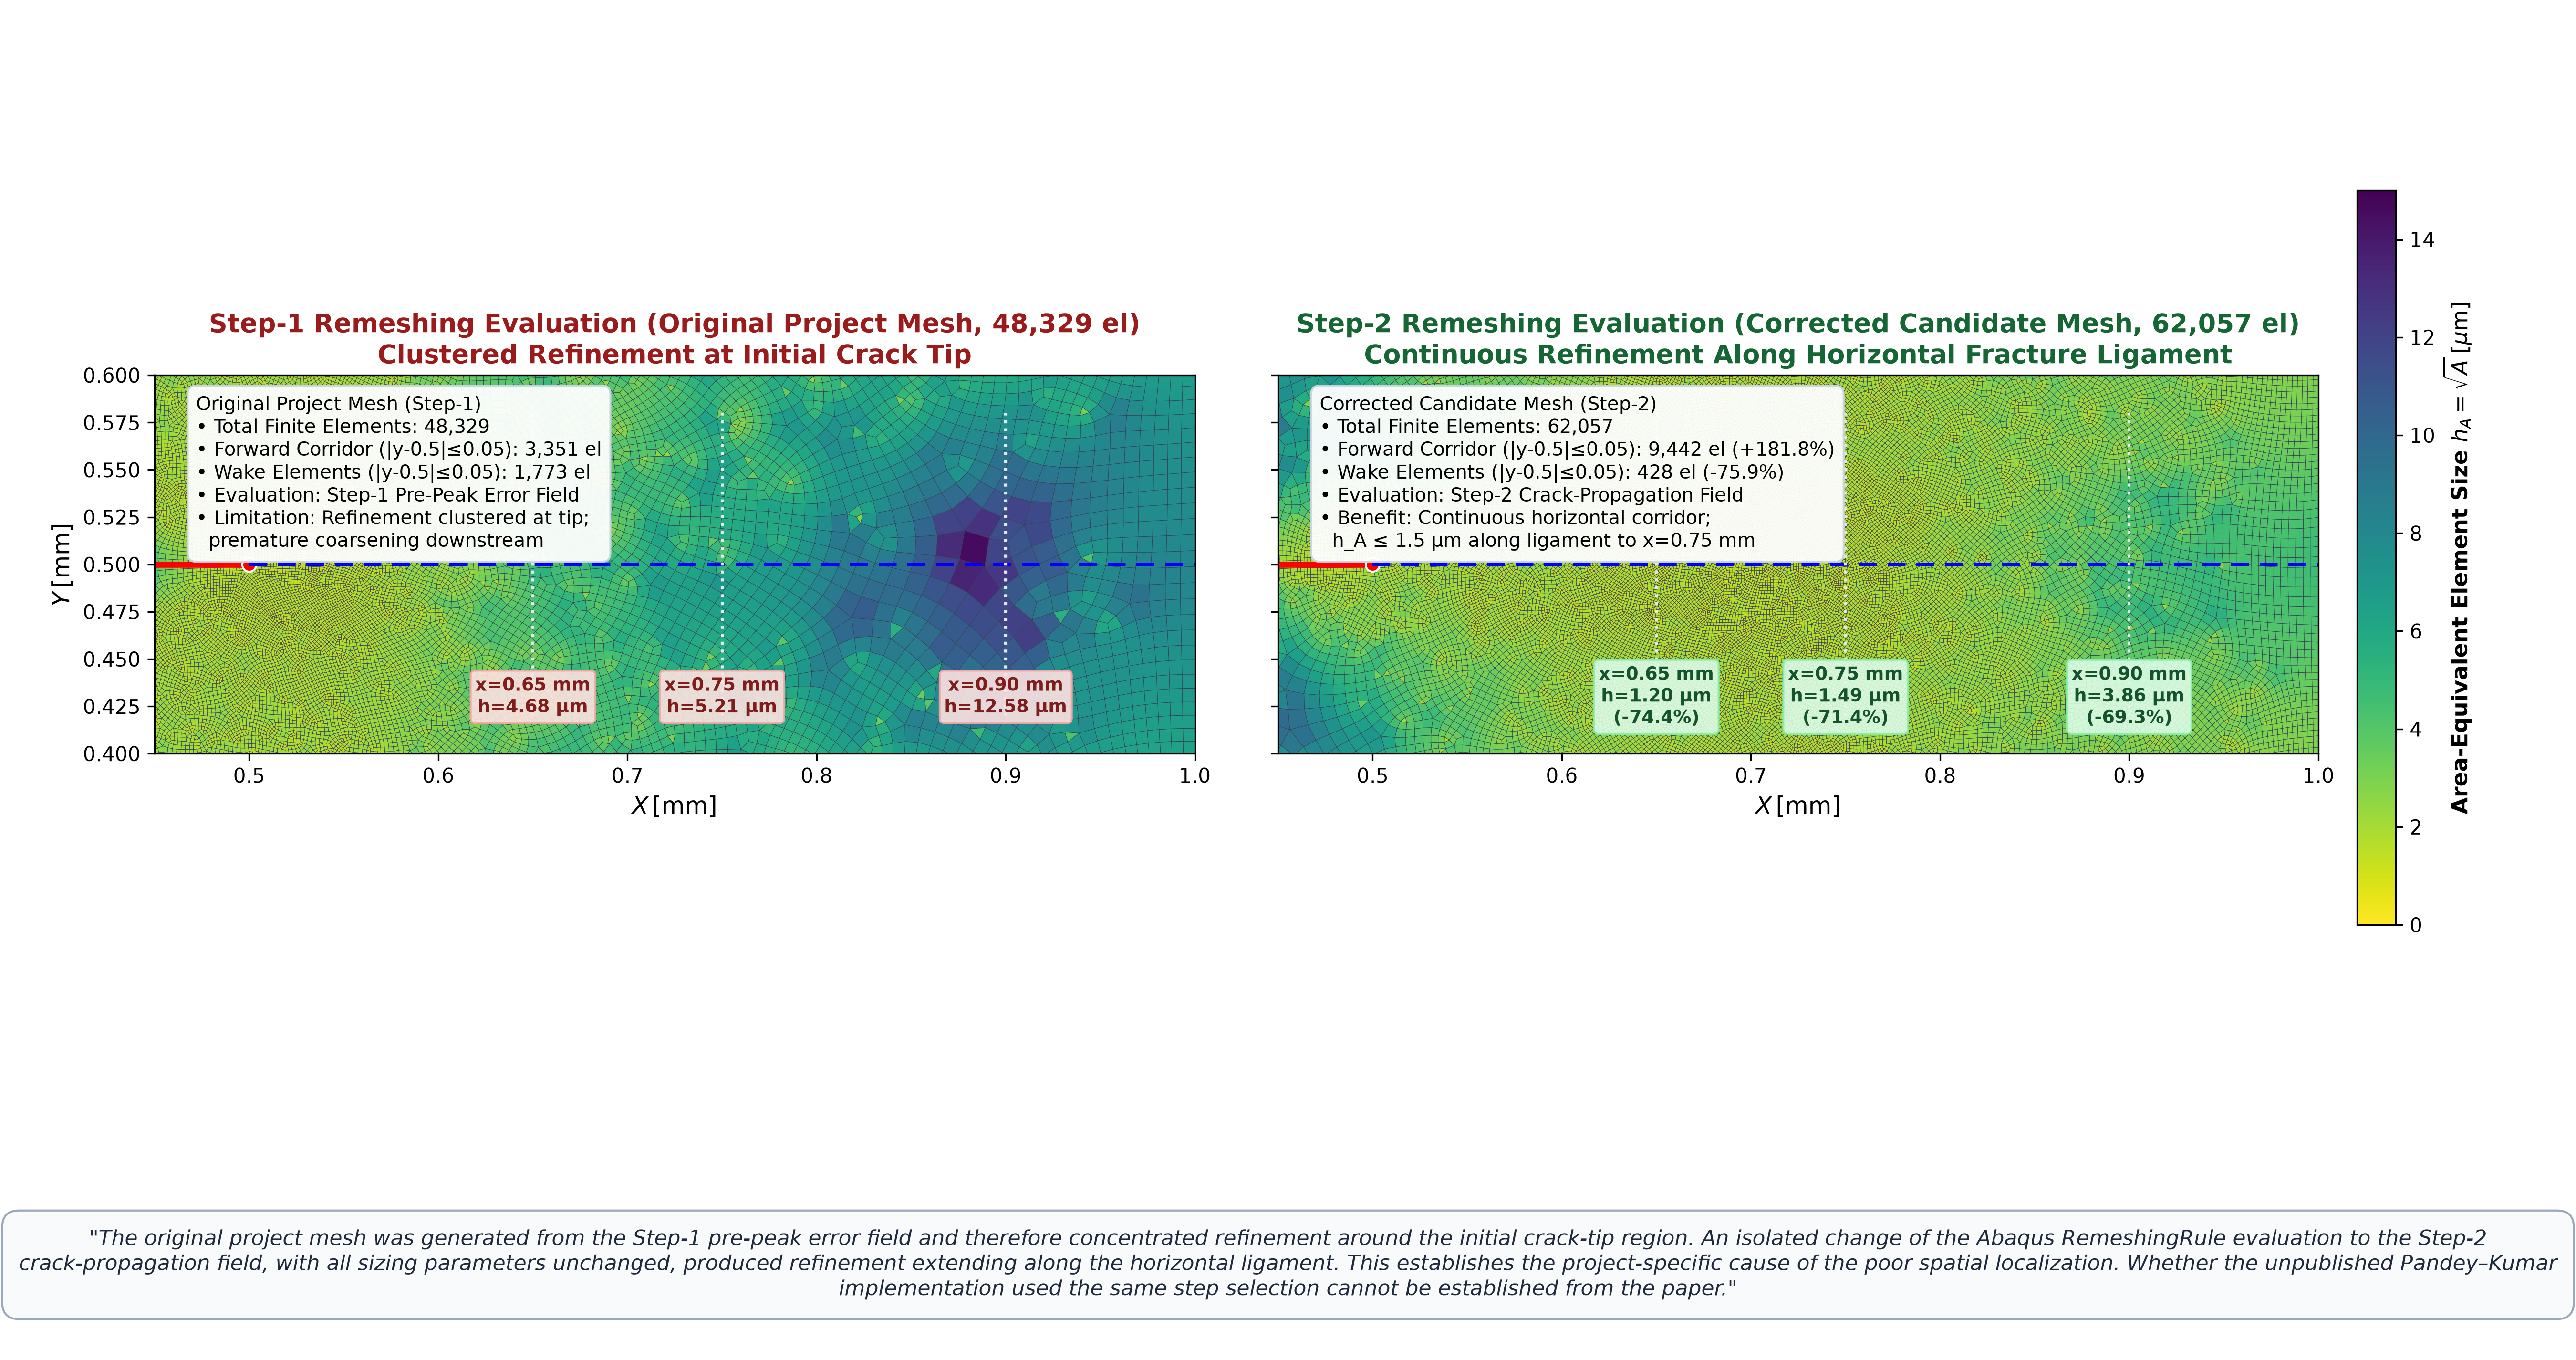
\includegraphics[width=0.88\textwidth]{figures/fig_step1_vs_step2_comparison.png}\\[0.1em]
  {\scriptsize\textbf{Figure 1:} Side-by-side comparison: Step-1 pre-peak evaluation ($48{,}329$ el) vs Step-2 crack-propagation evaluation ($62{,}057$ el).}
\end{center}

\clearpage

% ==================== PAGE 2 ====================
\vspace*{-0.3em}
\begin{center}
  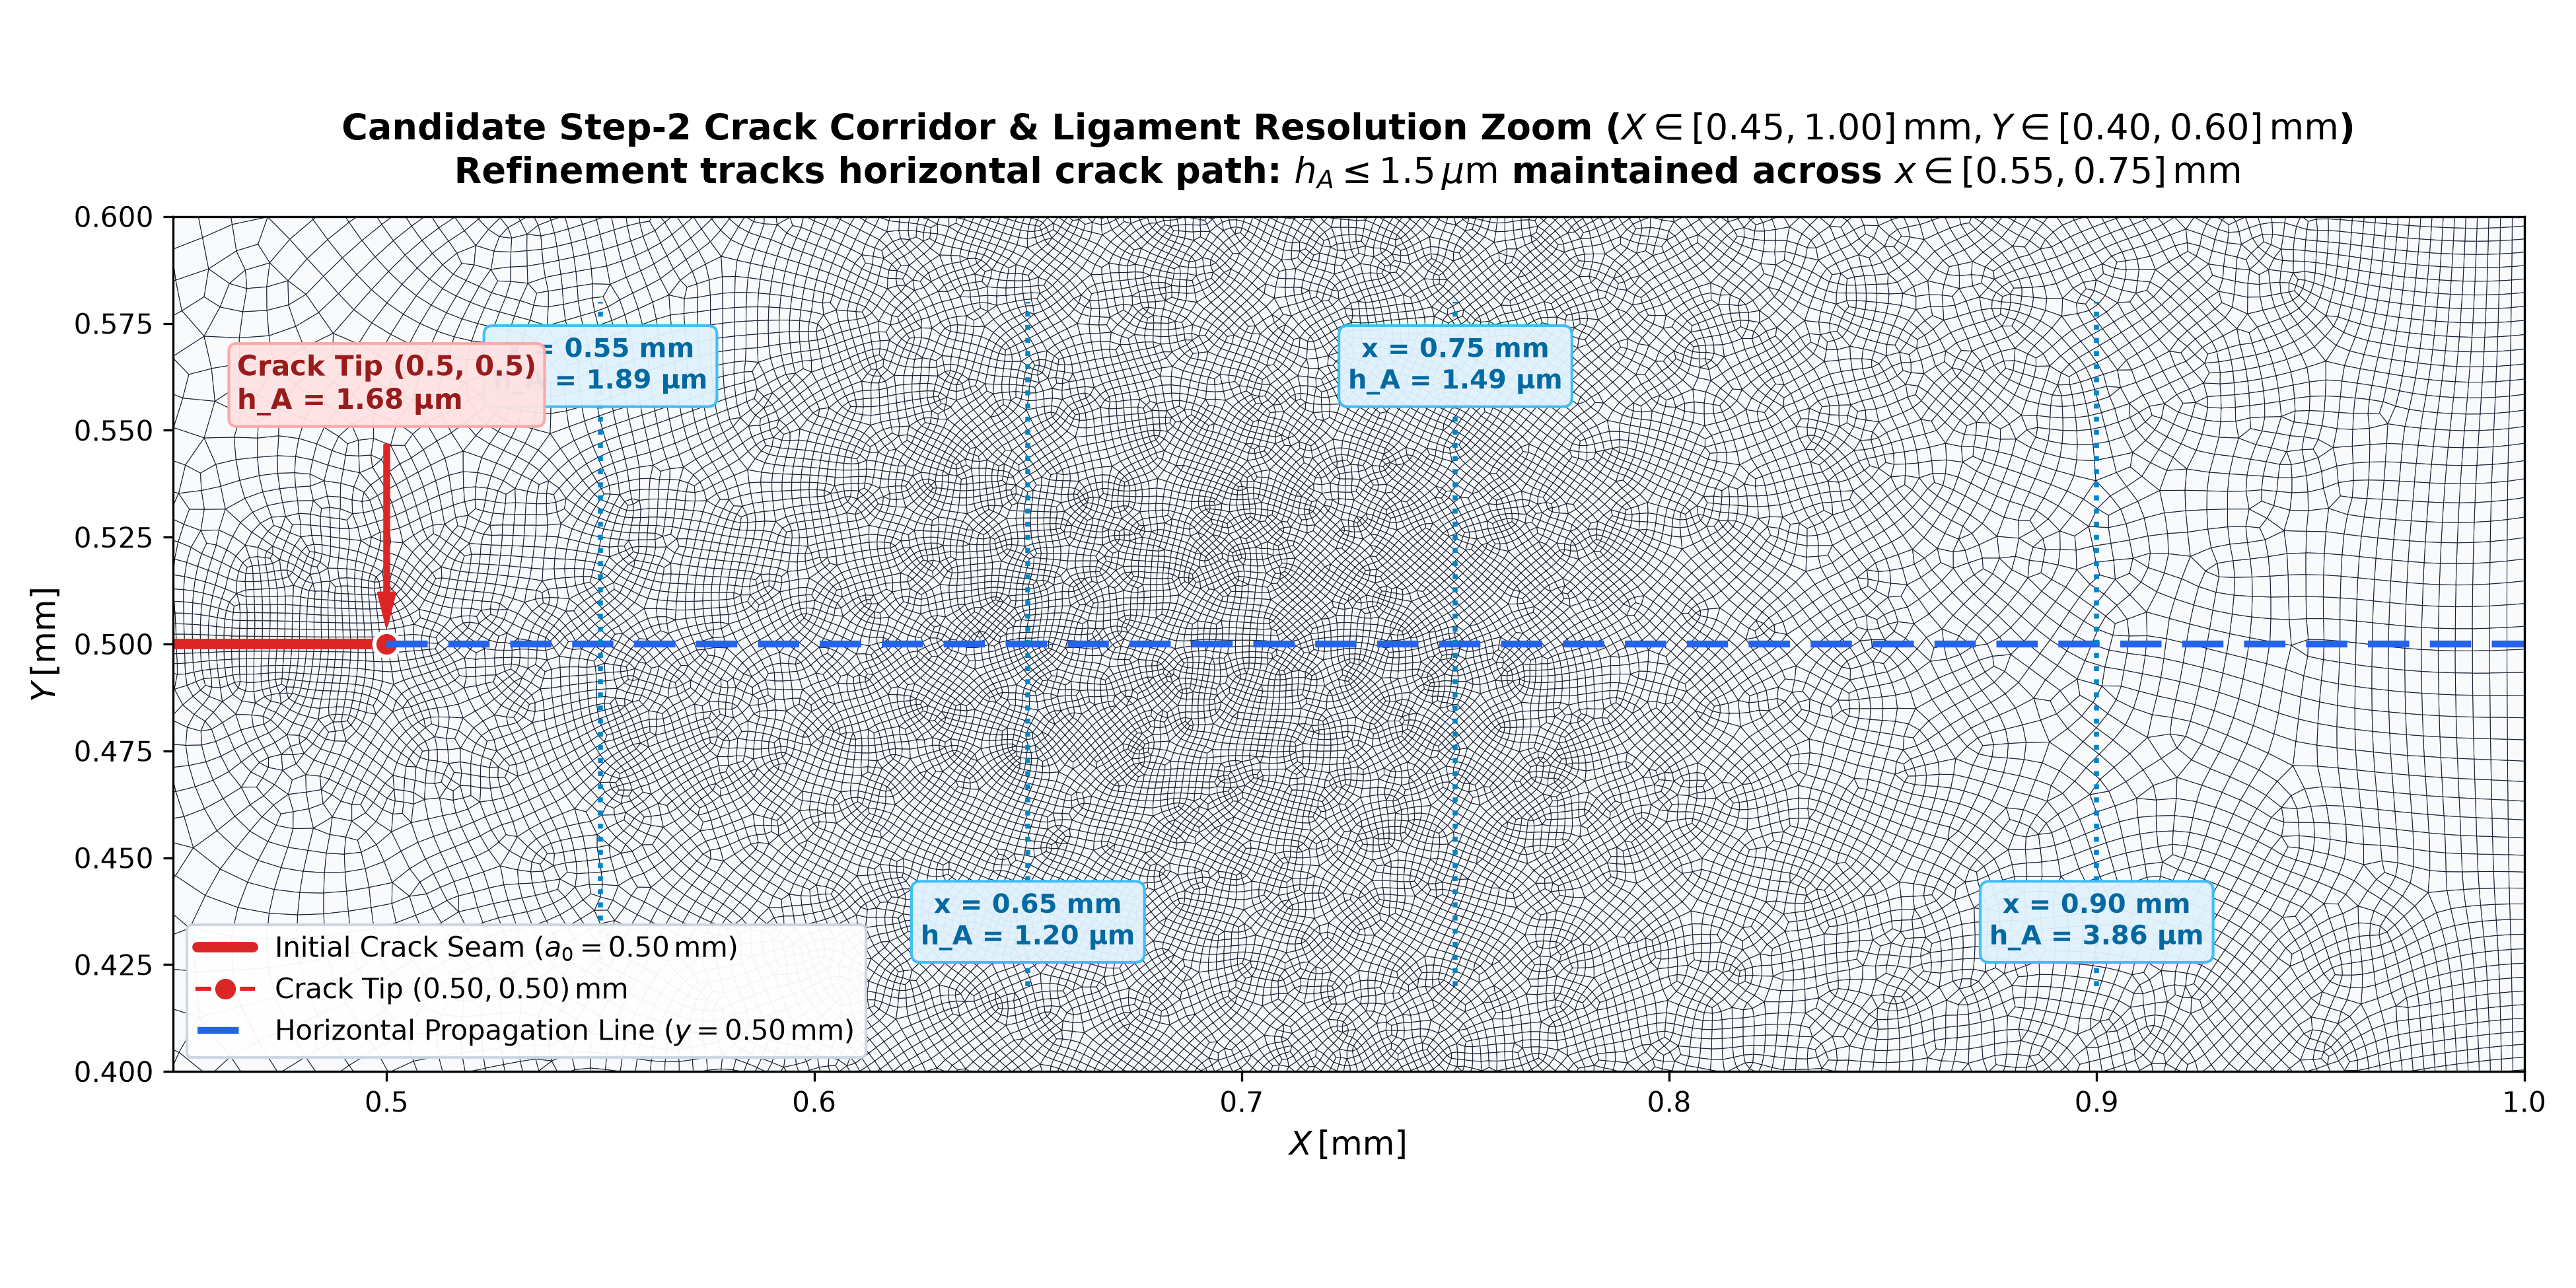
\includegraphics[width=0.74\textwidth]{figures/fig_step2_mesh_zoom.png}\\[0.1em]
  {\scriptsize\textbf{Figure 2:} Step-2 crack-corridor zoom ($y \in [0.45, 0.55]\,\mathrm{mm}$) with downstream cut stations $x \in \{0.55, 0.65, 0.75, 0.90\}\,\mathrm{mm}$.}
\end{center}

\vspace{-0.35em}
\subsection*{4. Epistemological Boundary: What is NOT Known}
\vspace{-0.25em}
\begin{tcolorbox}[colback=yellow!8!white,colframe=orange!80!black,title=\textbf{Epistemological Separation: Project Root Cause vs Published Methodology},top=2pt,bottom=2pt,left=4pt,right=4pt]
\small
\begin{itemize}[itemsep=0.6pt,topsep=0.2pt,leftmargin=4mm]
  \item \textbf{VERIFIED PROJECT ROOT CAUSE:} Within our Abaqus Python workflow, evaluating \texttt{RemeshingRule} on Step-1 vs Step-2 error fields is the verified technical cause that governs tip clustering vs full ligament refinement.
  \item \textbf{UNKNOWN AUTHOR IMPLEMENTATION DETAIL:} Pandey \& Kumar (2025, Sec.~4.1) state only that a remeshing rule was created based on \texttt{MISESERI} at $1\%$, omitting all script-level \texttt{stepName} or frame arguments. We \textbf{cannot and do not claim} that Pandey \& Kumar used Step 2. Their exact internal selection remains an unresolvable author implementation detail.
\end{itemize}
\end{tcolorbox}

\vspace{-0.25em}
\subsection*{5. Mechanical Status \& Output-Provenance Audit (Job 1409585.mmaster02)}
\vspace{-0.25em}
Spatial corridor refinement is \textbf{necessary but not sufficient} for scientific adoption:
\begin{itemize}[itemsep=0.3pt,topsep=0.2pt,leftmargin=4mm]
  \small
  \item \textbf{Status:} \texttt{ROOT\_CAUSE\_CANDIDATE\_NOT\_YET\_RECONCILED} (\textbf{Zero replacement jobs authorized}).
  \item \textbf{Mechanical Progression:} Solved 213 increments ($u \to 0.006554\,\mathrm{mm}$) with an $87.9\%$ continuous load drop ($F: 0.741 \to 0.089\,\mathrm{kN}$), $K_0 = 137.84\,\mathrm{kN/mm}$ ($\Delta = -0.08\%$), and stable horizontal crack extension across $\mathbf{94.0\%}$ \textbf{of ligament} ($x(d \ge 0.5) = 0.9701\,\mathrm{mm}$, $x(d \ge 0.95) = 0.9513\,\mathrm{mm}$) with zero local anomalies.
  \item \textbf{Output Provenance Audit:} Traced phase field $d$ (UEL nodal DOF 3) and $\mathcal{H}$ to companion Layer~3 (\texttt{All\_elem}) $\mathrm{STATEV}(1..20)$. The fixed reference deck (\texttt{1398090.mmaster02}) requested only \texttt{DISP\_QUAD} and \texttt{N\_RP}, omitting \texttt{SDV} and mesh \texttt{U} fields; its spatial metrics are classified as \textbf{\texttt{NOT\_AVAILABLE\_FROM\_THIS\_ODB}} / \textbf{\texttt{UNAVAILABLE}} rather than false zeros.
  \item \textbf{Boundary Formulation \& Bounds:} Decks prescribe displacement boundary conditions only; there is \textbf{no explicit phase-field Dirichlet condition}. The weak form implies natural zero-flux ($\partial d/\partial n = 0$). Peak phase field reaches $d_{\max} = 1.0008$ ($+8\times 10^{-4}$ overshoot above unity); \texttt{f42\_mixed\_uel.for} does not clip $d$, producing an approximately bounded continuous solution.
  \item \textbf{Diagnostics \& Matrix Revision:} MSG scan confirmed \textbf{0 negative eigenvalues, 0 singularities, 0 zero-pivots, 0 distorted elements, and 0 warnings}. Termination was triggered solely by $\Delta t < 10^{-8}\,\mathrm{s}$ at final breach. \texttt{RIGHT\_BOUNDARY\_PHASE\_FIELD\_INTERACTION} is downgraded to \textbf{\texttt{INSUFFICIENT\_EVIDENCE}} (spatial correlation with advancing crack tip, unproven boundary causation).
\end{itemize}

\vspace{-0.25em}
\subsection*{6. Formal Supervisor Decision Requested}
\vspace{-0.25em}
We request a ruling from the supervisors on the baseline strategy for the Master's thesis:

\begin{tcolorbox}[colback=green!5!white,colframe=green!60!black,title=\textbf{Option A: Adopt Step-2 Mesh as Baseline for Spatial Localization (Recommended)},top=2pt,bottom=2pt,left=4pt,right=4pt]
\small
Formally designate the $62{,}057$-element Step-2 adapted mesh as the thesis Mode-I Adaptive Baseline for spatial localization, documenting in Chapter~3 that Step-2 evaluation is required to achieve ligament localization under Abaqus native error indicators, while treating final breakthrough termination as a documented numerical open item.
\end{tcolorbox}

\vspace{-0.15em}
\begin{tcolorbox}[colback=gray!5!white,colframe=gray!60!black,title=\textbf{Option B: Retain Step-1 as Literal Reproduction Baseline; Present Step-2 as Project Improvement},top=2pt,bottom=2pt,left=4pt,right=4pt]
\small
Retain the $48{,}329$-element Step-1 mesh in Chapter~3 as the literal reproduction baseline resulting from strict pre-peak error evaluation, and present the $62{,}057$-element Step-2 mesh in Chapter~7 as an author-developed methodology correction that resolves the spatial localization deficit.
\end{tcolorbox}

\vfill
\hrule height 0.4pt
\vspace{0.12em}
{\scriptsize\textbf{Artifact Hashes:} Raw Mesh: \texttt{DA50340F...} $\cdot$ UEL Deck: \texttt{83C31D0D...} $\cdot$ Inspection Package: \texttt{exports/Mode1\_step2\_corrected\_mesh/}}

\end{document}
